%% IMPORTANT: Once working, run latex 3 times to get listoffigures to work

%% Be sure to check spelling!

%% Put ***your*** name and the proper due date in place

%% Note put your own file names in the appendix
%% Copy the relevant code as many times as needed for all files

%% Note that the \epsfig command is currently commented out

\documentclass{article}
\usepackage{amsmath}    % load AMS-Math package
\usepackage{epsfig}     % allows PostScript files
\usepackage{listings}   % allows lstlisting environment
\usepackage{moreverb}   % allows listinginput environment
\usepackage{vmargin}    % allows better margins
\setpapersize{USletter} % sets the paper size
\setmarginsrb{1in}{0.5in}{1in}{0.2in}{12pt}{11mm}{0pt}{11mm} %sets margins 
\begin{document}
\begin{center}
\rule{6.5in}{0.5mm}\\~\\
{\bf \large EGR 103L -- Fall 2016}\\~\\
{\huge \bf Laboratory 6 - Roots and Extrema Problems}\\~\\
CEMAL YAGCIOGLU (cy111)\\
Lab Section 5D, Wednesday 11.45AM - 2.35PM\\
23 OCTOBER, 2016\\~\\
{\small I understand and have adhered to all the tenets of the Duke
  Community Standard in completing every part of this assignment.  I
  understand that a violation of any part of the Standard on any part
  of this assignment can result in failure of this assignment, failure
  of this course, and/or suspension from Duke University.} 
\rule{6.5in}{0.5mm}\\
\end{center}
\tableofcontents
\listoffigures
\pagebreak

\section{Basic Root-Finding Problems}
\begin{center}
\renewcommand{\arraystretch}{2.0}
\begin{tabular}{|c|c|c|}
\hline
Function & Real Roots & Roots\\\hline
$f(x)=20e^{-4x}-36e^{-2x}+18e^{-x}-1$ & 3 & 4.5651e-02, 6.3358e-01, 2,7545e+00\\\hline
$f(x)=x^5+100\mathrm{cos}(2x)$ & 3 & -7.8391e-01, 7.8691e-01, 2.1295e+00\\\hline
$f(x)=\frac{10}{x-2}-90e^{-(x/20)},x\neq2$ & 2 &  2.3620e+00, 7.9669e+00\\\hline
\end{tabular}
\end{center}


\section{Basic Min/Max-Finding Problems}
\begin{center}
\begin{tabular}{|c|c|c|}
\hline
Function & Counts & Extrema\\\hline
$f(x)=20e^{-4x}-36e^{-2x}+18e^{-x}-1$ & 1 min, 1 max & min:$f(2.4511e-01)=-1.4596e+00$\\
 & & max:$f(1.3002e+00)=1.3421e+00$\\\hline
$f(x)=x^5+100\mathrm{cos}(2x)$ & 2 min, 2 max & min 1:$f(-1.6682e+00)=-1.1103e+02$\\
 & & min 2:$f(1.5063e+00)=-9.1415e+01$\\
 & & max 1:$f(-2.4916e+00)=-6.9275e+01$\\
 & & max 2:$f(4.9908e-07)=1.0000e+02$\\\hline
\end{tabular}
\end{center}
 
\section{Chapra 6.16}
\begin{center}
\begin{tabular}{|c||c|c|c|c|c|c|}
\hline
$V$.$\mathrm{m}^{3}$ & 10 & 20 & 30 & 40 & 50 & 60\\\hline
$h$,m & 8.6492e-01 & 1.4210e+00 & 1.9292e+00 & 2.4326e+00 & 2.9685e+00 & 3.6373e+00\\\hline
\end{tabular}
\end{center}


\section{Chapra 6.21}
Angles are 37.959 and 51.532 degrees.

\section{Chapra 7.23, 7.24, and 7.25(b/c)}
For function 1, minimum value occurs at (x,y)=(5.6759e-01,7.5677e-01). The function''s value at this point is -6.6216e-01.
For function 2, max value occurs at (x,y)=(9.6759e-01,6.5589e-01). The function''s value at this point is 4.3440e+00.
For function 3, minimum value occurs at (x,y)=(3.3333e+00,-6.6670e-01). The functions value at this point is -1.7333e+01.
\pagebreak

\appendix
\section{Codes}
% Put the name of your file in the subsection name 
% and the listinginput input
% Be sure to include the community standard in codes!
% Add \pagebreaks if they make sense

% Put the files in the same order as the problems; generally, 
% scripts will come first followed by any functions called
% by those scripts.

\subsection{Roots.m}
\listinginput[1]{1}{Roots.m}


\subsection{HeightCylinder.m}
\listinginput[1]{1}{HeightCylinder.m}

\subsection{Projectile.m}
\listinginput[1]{1}{Projectile.m}

\subsection{ExtremeValue.m}
\listinginput[1]{1}{ExtremeValue.m}

\pagebreak


\section{Figures}
% Make as many as needed; change sizes if it makes sense to do so
%% For the first one, here is one way to have three plots:
\begin{figure}[htb!]
\begin{center}
\begin{tabular}{cc}
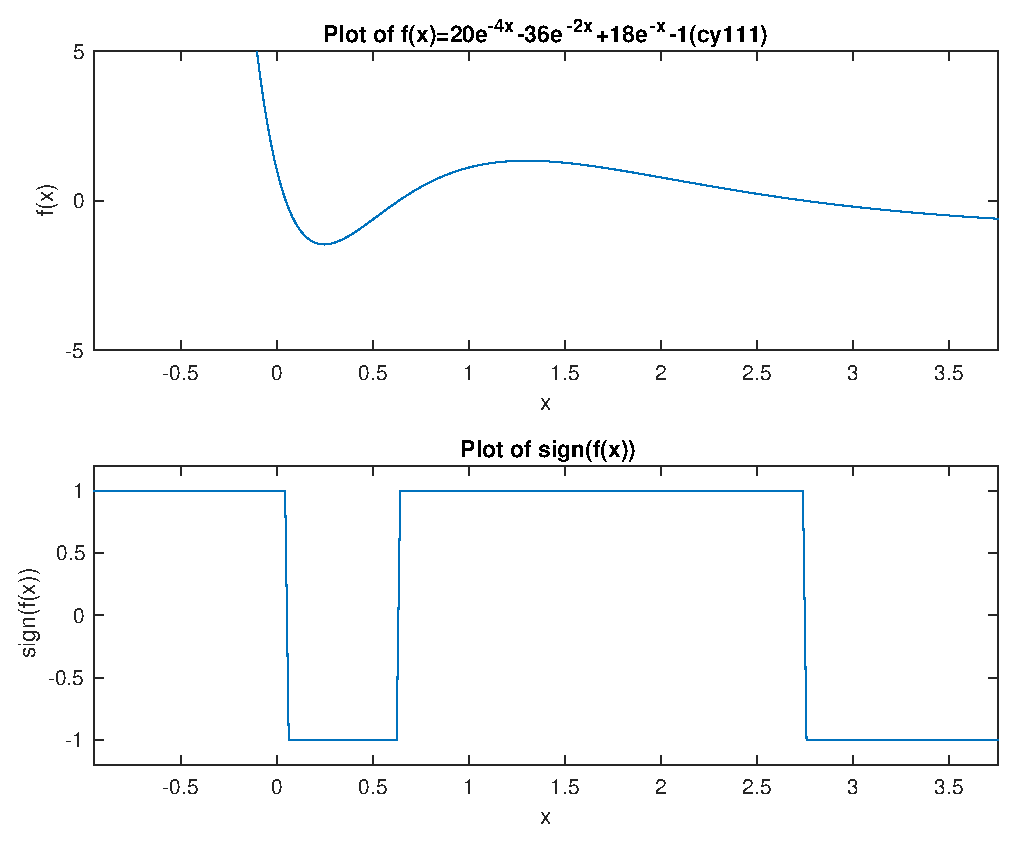
\epsfig{file=Roots1.eps, width=2.5in} &
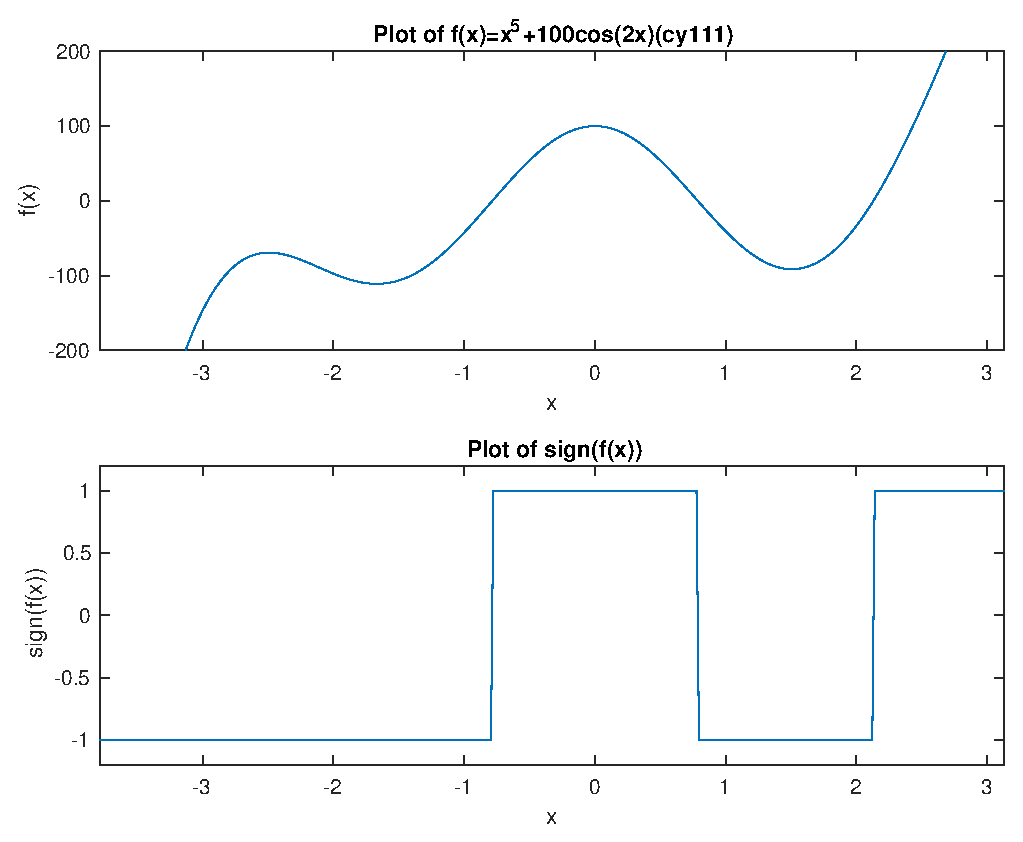
\epsfig{file=Roots2.eps, width=2.5in}\\
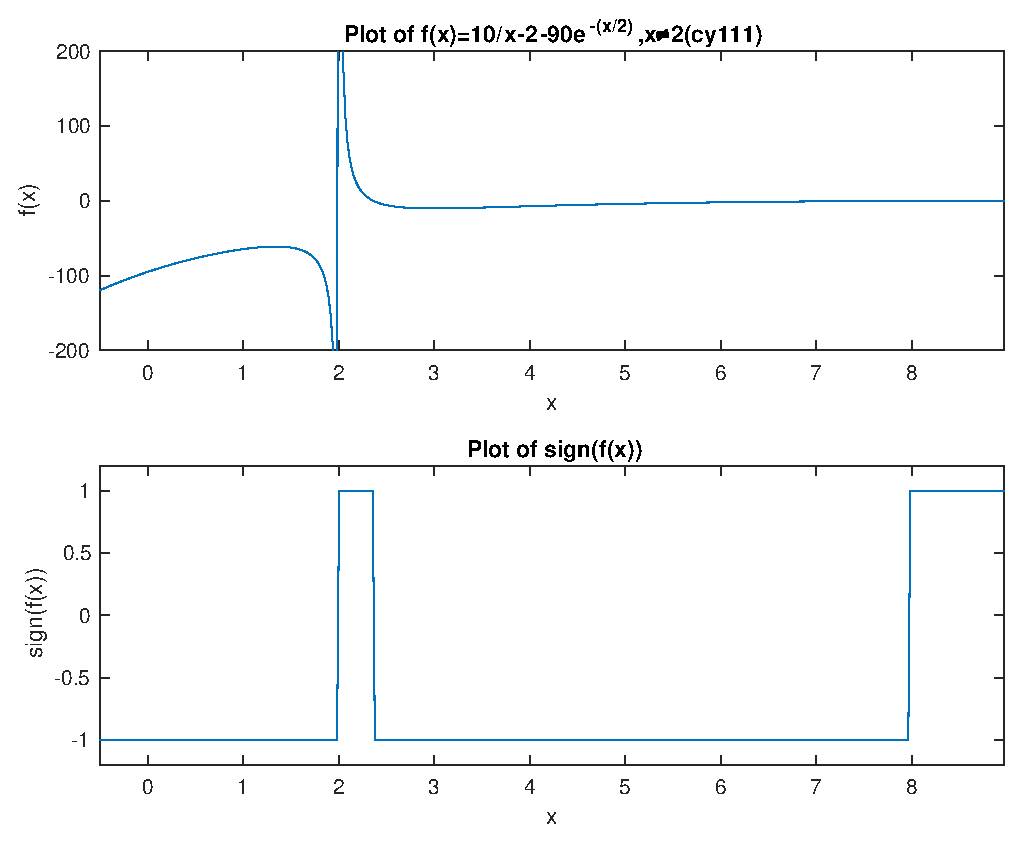
\epsfig{file=Roots3.eps, width=2.5in} &
~
\end{tabular}
\caption{Basic Roots Problems}
\end{center}
\end{figure}


\begin{figure}[htb!]
\begin{center}
\epsfig{file=ProjectileGraph.eps, width=4in}
\caption{Projectile Motion Problem}
\end{center}
\end{figure}


\begin{figure}[htb!]
\begin{center}
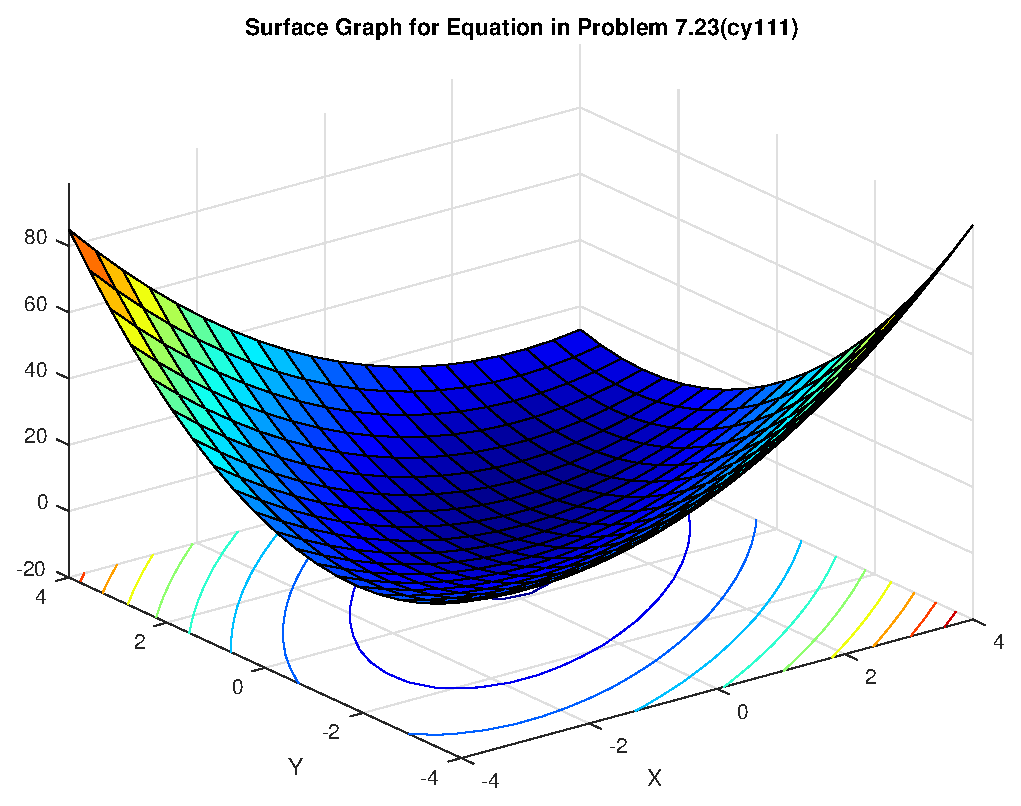
\epsfig{file=Surface1.eps, width=4in}
\caption{Max/Min Surface Graph 1}
\end{center}
\end{figure}


\begin{figure}[htb!]
\begin{center}
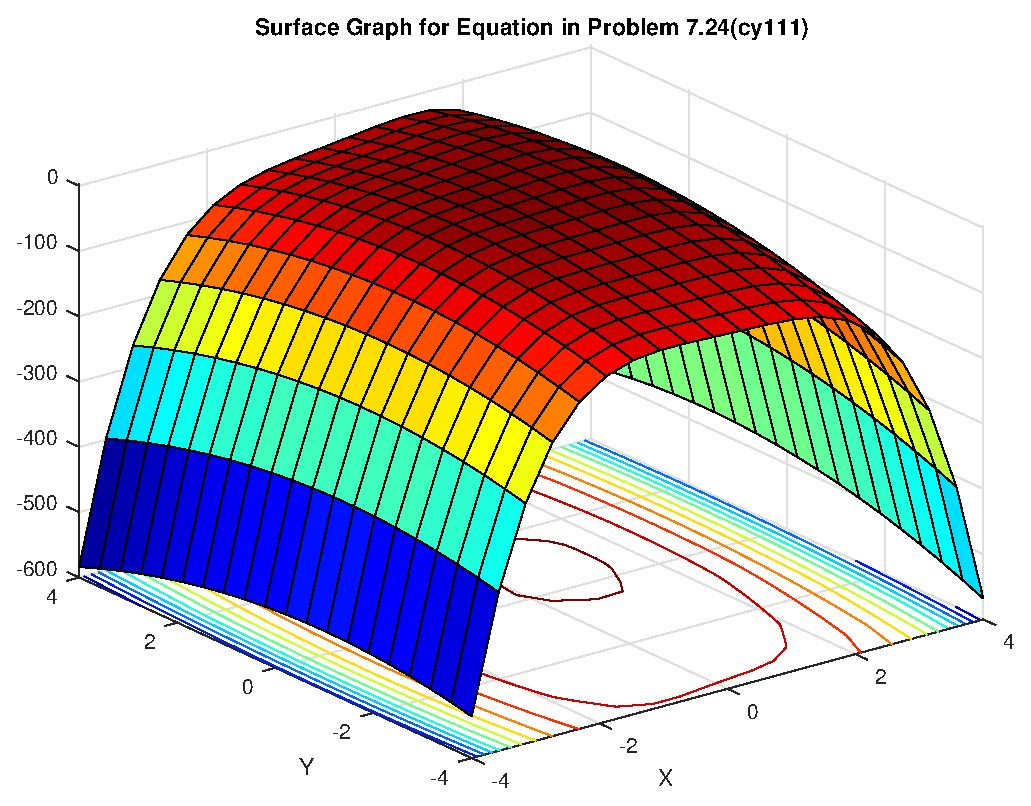
\epsfig{file=Surface2.eps, width=4in}
\caption{Max/Min Surface Graph 2}
\end{center}
\end{figure}


\begin{figure}[htb!]
\begin{center}
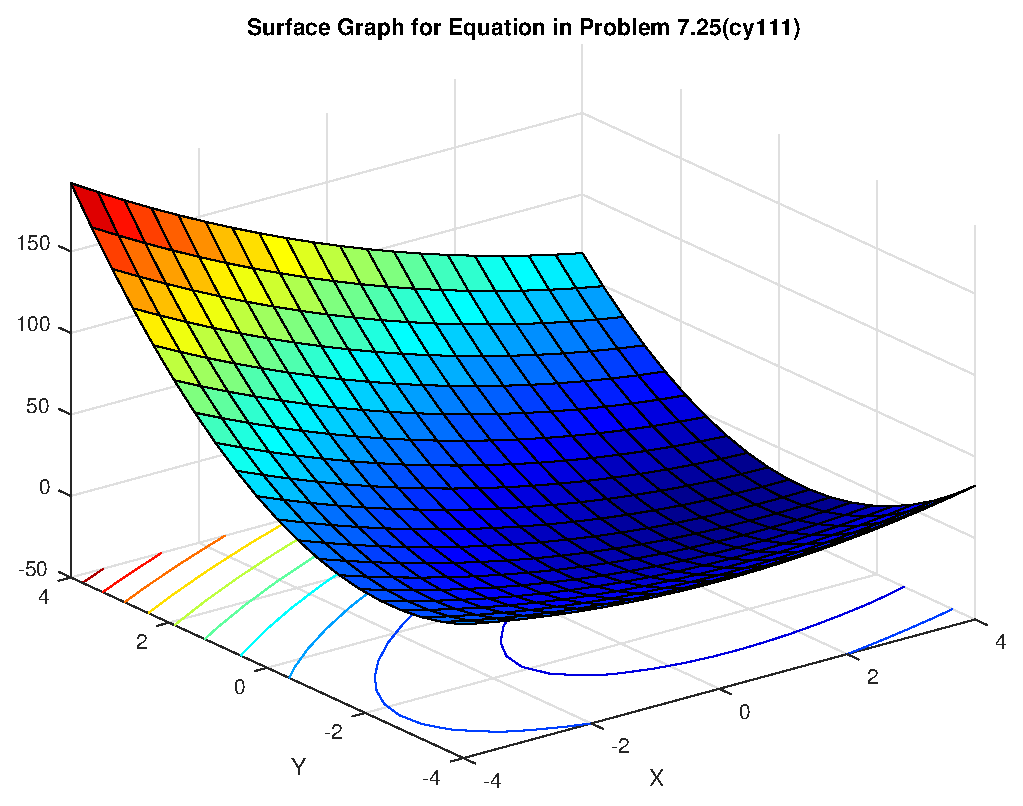
\epsfig{file=Surface3.eps, width=4in}
\caption{Max/Min Surface Graph 3}
\end{center}
\end{figure}



\end{document}
